\section{Benchmarks}

Des tests de performance ont été réalisés sur les deux versions de la fonction \texttt{getrf()} : version par bloc et version MPI. Les deux sont très similaires et les tests sont donc les mêmes : une matrice aléatoire de taille carrée (par défaut 512) est allouée puis factorisée avec un certaine taille de bloc. L'opération est recommencée un certain nombre de fois pour assurer la cohérence des valeurs (ici $4$ fois) puis le programme passe à l'itération suivante avec une taille de bloc supérieure, incrémentée d'un cinquième. Le temps d'exécution comprend uniquement le temps de factorisation du thread $0$, ne tendant pas compte donc de la répartition de la matrice sur les processus.

Nous n'arrivons pas à trouver d'explication satisfaisante concernant la diminution du temps de calcul lorsque la taille des blocs augmente, et ce pour toutes les version, quelque que soit le nombre de processus. Ce phénomène est visible sur tous les résultats ci-dessous, au plus tard à partir d'une taille de bloc égale à la moitiée de la matrice. Nous pensions que le temps d'exécution devait augmenter en même temps que la taille des blocs.

Cependant les graphiques \ref{fig:d_2} et \ref{fig:d_4} révèlent l'effet de cache pour des tailles de bloc d'environ $50$ et $125$ où se trouvent des pics de rapidité du temps d'exécution. Nous supposons que ces tailles de bloc correspondent à plus ou moins à la taille des caches, ce qui est difficile à vérifier car la fonction de factorisation possède en dehors de sa partie locale de la matrice deux autres matrices : la dernière colonne \emph{broadcasté} et la dernier bloc factorisé. Toutefois les tailles de blocs mentionnées correspondent respectivement à $50 \times 50 \times 8 = 20 ko$ et $125 \times 125 \times 8 = 125 ko$ puisque nous utilisons le type \texttt{double} qui est codé sur $8$ octets. Or les tailles de cache de Plafrim sont justement légèremet supérieures à ces valeurs : $32 ko$ pour le L1 et $256$ pour le L2, les effets observés sont donc vraissemblablement des effets de caches : les blocs de taille $50$ et $125$ sont ceux de taille maximum qui rentrent respectivement dans le L1 et le L2. Une incrémentation plus fine des tailles de blocs pourraient certaintement certifier cette hypothèse.

\begin{figure}
\centering
\begin{subfigure}[b]{0.48\textwidth}
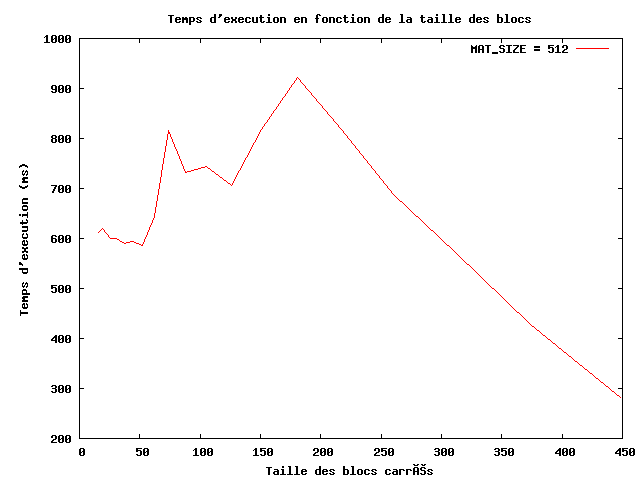
\includegraphics[width=\textwidth]{data_dgetrf_2.png}
\caption{2 processus}
\label{fig:d_2}
\end{subfigure}
\begin{subfigure}[b]{0.48\textwidth}
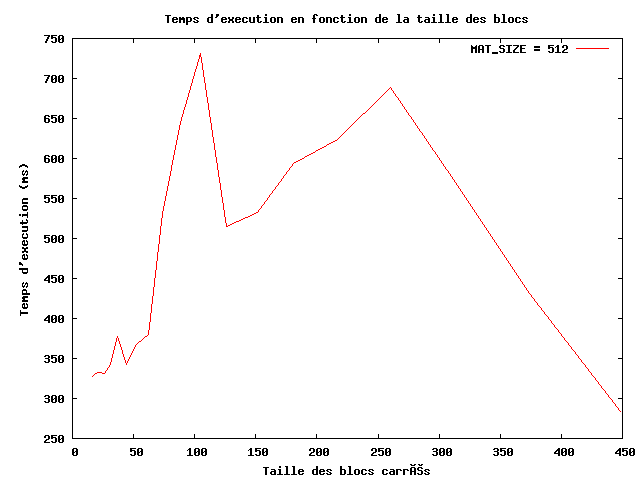
\includegraphics[width=\textwidth]{data_dgetrf_4.png}
\caption{4 processus}
\label{fig:d_4}
\end{subfigure}

\begin{subfigure}[b]{0.48\textwidth}
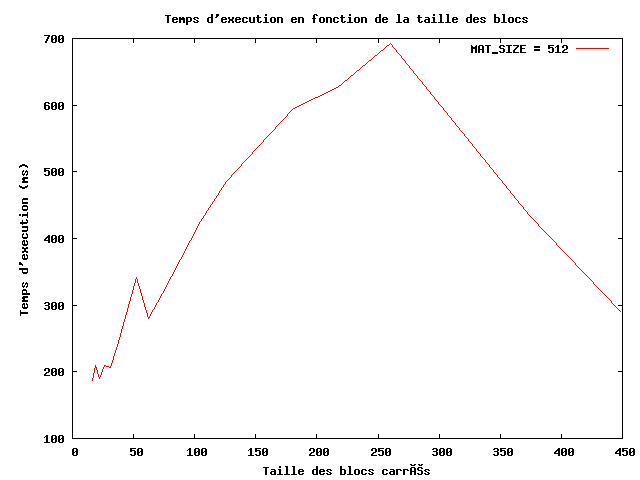
\includegraphics[width=\textwidth]{data_dgetrf_8.png}
\caption{8 processus}
\label{fig:d_8}
\end{subfigure}
\begin{subfigure}[b]{0.48\textwidth}
\centering
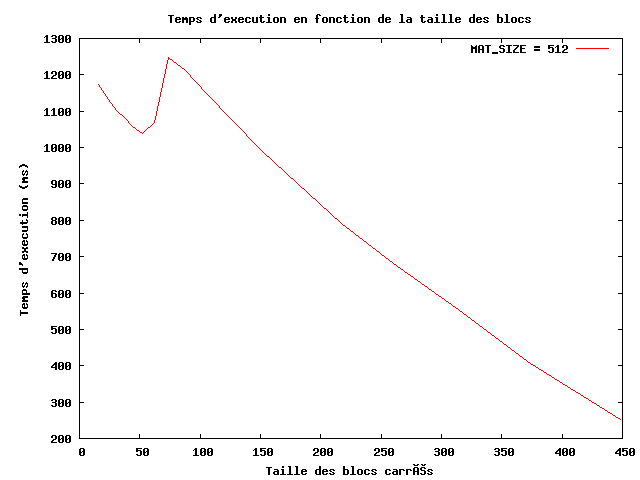
\includegraphics[width=\textwidth]{data_dgetrf_seq.png}
\caption{version séquentielle}
\label{fig:d_s}
\end{subfigure}
\caption{Temps d'exécution en fonction de la taille des blocs, pour un nombre différent de processus.}
\end{figure}

